\documentclass{article}
\usepackage{tikz, pgf-pie, tcolorbox}
\usetikzlibrary{arrows.meta}
\tikzset{>=Triangle}
\usepackage[margin=2cm, a4paper]{geometry}

\usepackage{hyperref}
\begin{document}
\tcbset{coltitle=black}
\begin{center}
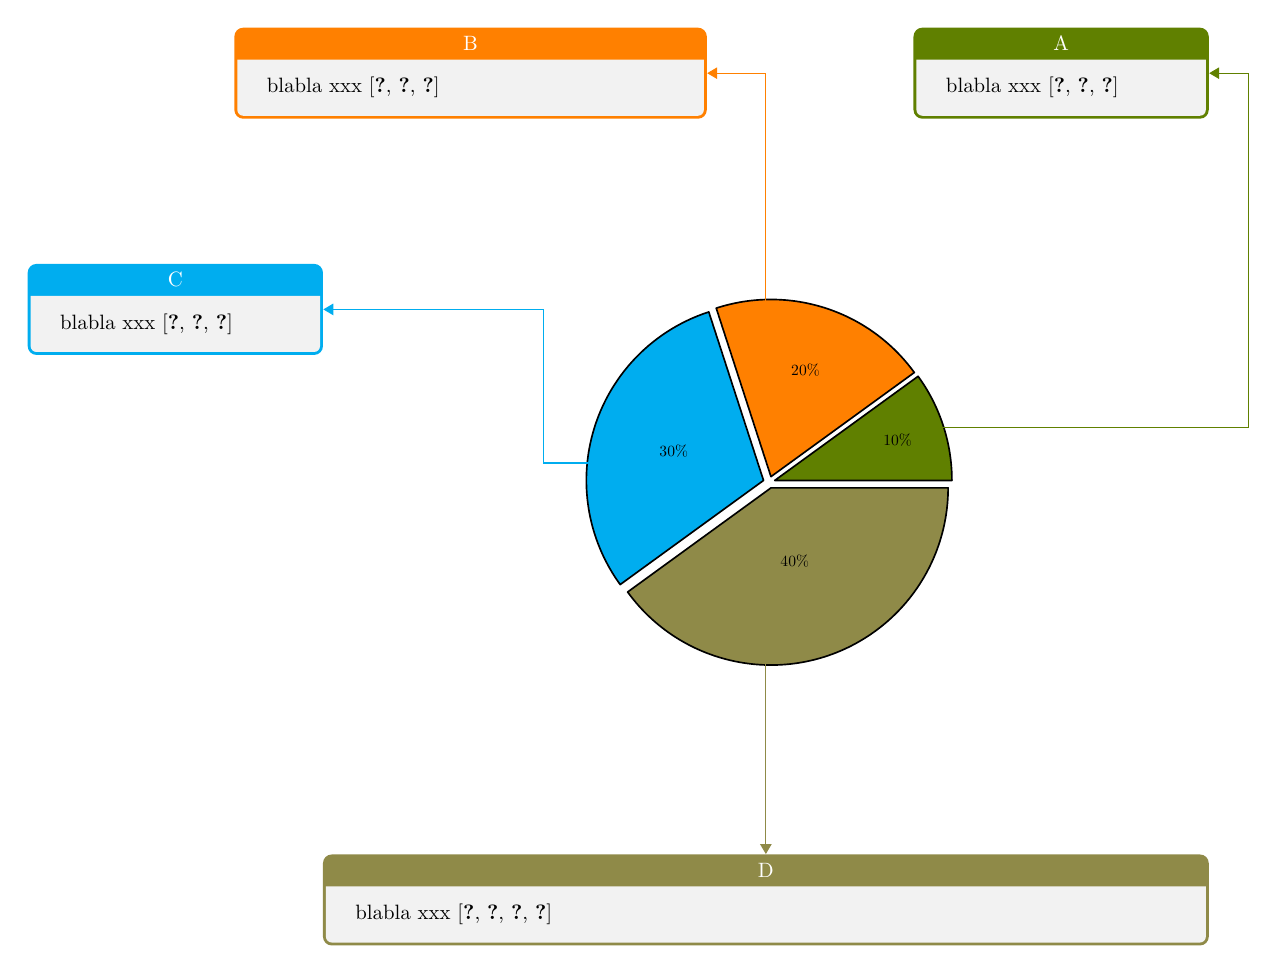
\begin{tikzpicture}[scale = .75, every node/.style={scale = .75}]
    \node[inner sep = 0pt] (pie) at (0,0) {
        \tikz {\pie[
            pos = {0,0}, 
            explode={0.1},
            color = {lime!50!black, orange, cyan, yellow!50!black},
        ]{10/, 20/, 30/, 40/}}
    };
    
    
    \node[text width = 5cm, inner sep = 0pt,] (A) at (5, 7) {
        \begin{tcolorbox}[title = A, center title, colframe = lime!50!black, before skip = 0pt]
            blabla xxx \cite{bishop2006pattern,chollet2015keras,knuth1984tex}
        \end{tcolorbox}
    };

    \node[text width = 8cm, inner sep = 0pt] (B) at (-5, 7) {
        \begin{tcolorbox}[title = B, center title, colframe = orange, before skip = 0pt]
            blabla xxx \cite{bishop2006pattern,russell2016ai,devlin2019bert}
        \end{tcolorbox}
    };

    \node[text width = 5cm, inner sep = 0pt] (C) at (-10, 3) {
        \begin{tcolorbox}[title = C, center title, colframe = cyan, before skip = 0pt]
            blabla xxx \cite{lamport1994latex,vaswani2017attention,lecun2015deep}
        \end{tcolorbox}
    };

    \node[text width = 15cm, inner sep = 0pt] (D) at (0, -7) {
        \begin{tcolorbox}[title = D, center title, colframe = yellow!50!black, before skip = 0pt]
            blabla xxx \cite{lamport1994latex,vaswani2017attention,lecun2015deep,russell2016ai}
        \end{tcolorbox}
    };

    \draw[cyan, ->] ([shift = {(0.4, 0.4)}]pie.west) -- ++ (-1, 0) |- (C.east);

    \draw[orange, ->] ([shift = {(0, -.5)}]pie.north) |- (B.east);

    \draw[lime!50!black, ->] ([shift = {(-.5, 1)}]pie.east) --++ (5.5,0) |- (A.east);

    \draw[yellow!50!black, ->] ([shift = {(0, 1)}]pie.south) -- (D.north);
\end{tikzpicture}
\end{center}


\begin{thebibliography}{10}

\bibitem{knuth1984tex}
Donald E. Knuth.
\newblock The {\TeX}book.
\newblock Addison-Wesley, 1984.

\bibitem{lamport1994latex}
Leslie Lamport.
\newblock {\LaTeX}: A Document Preparation System.
\newblock Addison-Wesley, 2nd edition, 1994.

\bibitem{goodfellow2016deep}
Ian Goodfellow, Yoshua Bengio, and Aaron Courville.
\newblock Deep Learning.
\newblock MIT Press, 2016.

\bibitem{russell2016ai}
Stuart Russell and Peter Norvig.
\newblock Artificial Intelligence: A Modern Approach.
\newblock Pearson, 3rd edition, 2016.

\bibitem{bishop2006pattern}
Christopher M. Bishop.
\newblock Pattern Recognition and Machine Learning.
\newblock Springer, 2006.

\bibitem{he2016resnet}
Kaiming He, Xiangyu Zhang, Shaoqing Ren, and Jian Sun.
\newblock Deep residual learning for image recognition.
\newblock In *Proceedings of the IEEE Conference on Computer Vision and Pattern Recognition (CVPR)*, 2016.

\bibitem{vaswani2017attention}
Ashish Vaswani et al.
\newblock Attention is all you need.
\newblock In *Advances in Neural Information Processing Systems (NeurIPS)*, 2017.

\bibitem{lecun2015deep}
Yann LeCun, Yoshua Bengio, and Geoffrey Hinton.
\newblock Deep learning.
\newblock *Nature*, 521(7553):436--444, 2015.

\bibitem{devlin2019bert}
Jacob Devlin, Ming-Wei Chang, Kenton Lee, and Kristina Toutanova.
\newblock BERT: Pre-training of deep bidirectional transformers for language understanding.
\newblock In *Proceedings of NAACL-HLT*, 2019.

\bibitem{chollet2015keras}
François Chollet.
\newblock Keras.
\newblock https://keras.io, 2015.

\end{thebibliography}

\end{document}